\subsubsection*{\underline{\textsc{\Large Time Guardian}}}
\noindent\emph{Medium construct, neutral}

The time guardian lives outside of normal time and space.

\noindent\rule{0.5\textwidth}{0.5pt}

\noindent\textbf{Armor Class}: 13

\noindent\textbf{Hit Points}: 54 (10d8+10)

\noindent\textbf{Speed}: 30 ft.

\noindent\rule{0.5\textwidth}{0.5pt} \\
\begin{table}[H]
	\begin{tabular}{cccccc}
		\textbf{STR} & \textbf{DEX} & \textbf{CON} & \textbf{INT} & \textbf{WIS} & \textbf{CHA} \\
		18 (+4) & 8 (-1) & 16 (+3) & 7 (-2) & 10 (+0) & 3 (-4) \\
	\end{tabular}
\end{table}
\noindent\rule{0.5\textwidth}{0.5pt} \\

\noindent\textbf{Damage Resistances}: acid, fire, lightning, thunder

\noindent\textbf{Damage Immunities}: cold, necrotic, poison

\noindent\textbf{Condition Immunities}: charmed, exhaustion, frightened, paralyzed, poisoned

\noindent\textbf{Senses}: darkvision 60 ft., passive Perception 11

\noindent\textbf{Languages}: Does not speak

\noindent\textbf{Challenge}: 4 (1,100 XP)

\noindent\rule{0.5\textwidth}{0.5pt}

\noindent\textbf{ACTIONS}

\noindent\textbf{Time's Grasp}: Melee Weapon Attack: +5 to hit, reach 5 ft., one target. Hit: 17 (4d6 + 3) necrotic damage. Targets hit by time's grasp must succeed a DC 12 constitution saving throw or experience rapid aging of the affected body part (determined by a d10, doesn't stack), permanently (a \textbf{potion of time rejuvenation} can be used to heal the affected area).

\begin{table}[H]
	\begin{tabular}{cll}
		\textbf{d10} & \textbf{Area} & \textbf{Effect} \\
		1-4 & Legs & Movement speed is halved \\
		5-7 & Chest & AC is reduced by 2 \\
		8-9 & Arms & Has disadvantage on attack rolls \\
		10 & Head & Has disadvantage on all rolls \\
	\end{tabular}
\end{table} 

\begin{center}
	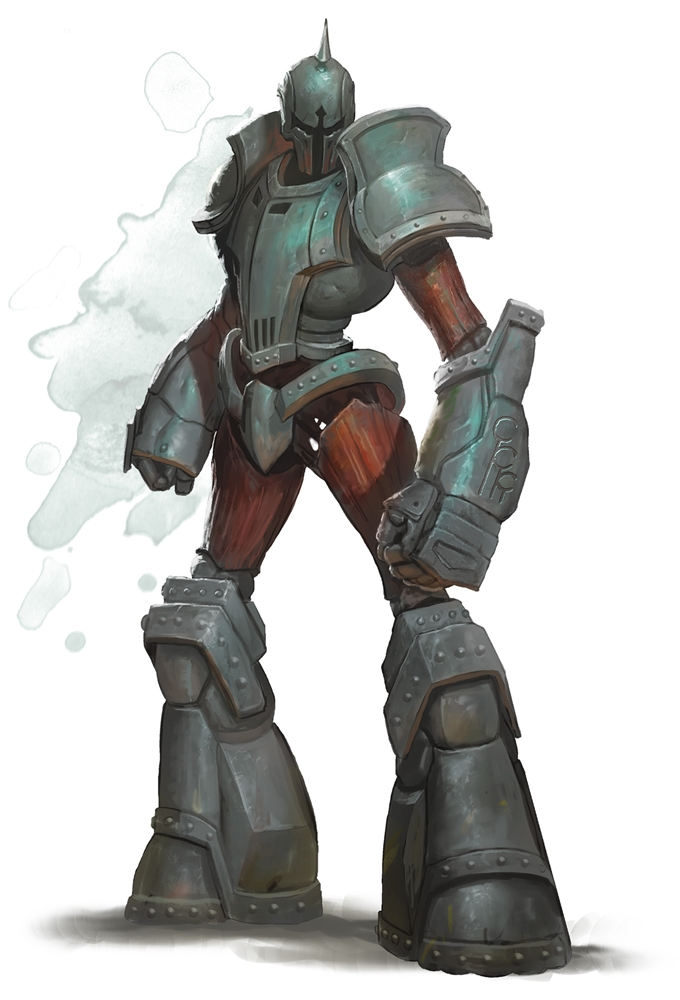
\includegraphics[width = 0.3\textwidth]{time-guardian}
	
	\emph{Time Guardian}
\end{center}